\begin{frame}
  \frametitle{What is software?}
  \begin{figure}[htpb]
      \centering
      \begin{subfigure}
        \centering
        
\includegraphics[width=1.5cm]{images/firefox-logo.png}
      \end{subfigure}
      \begin{subfigure}
        \centering
        
\includegraphics[width=5cm]{images/openmc-logo.png}
      \end{subfigure}
      \begin{subfigure}
        \centering
        
\includegraphics[width=2cm]{images/git-logo.png}
      \end{subfigure}
      \newline
      {\tiny Sources: \cite{firefox_logo}, \cite{openmc_logo}, \cite{git_logo}}
  \end{figure}
  % a comment
  % add photos of software
  % firefox, openmc, etc
  \pause\medskip
  \begin{itemize}
      \item Ultimately, software is a {\it tool} we can use to solve complex problems.
  \end{itemize}
\end{frame}

\begin{frame}
    \frametitle{What kinds of problems do {\it we} use software to solve?}

    \begin{figure}[htpb]
        \begin{subfigure}
            \centering
            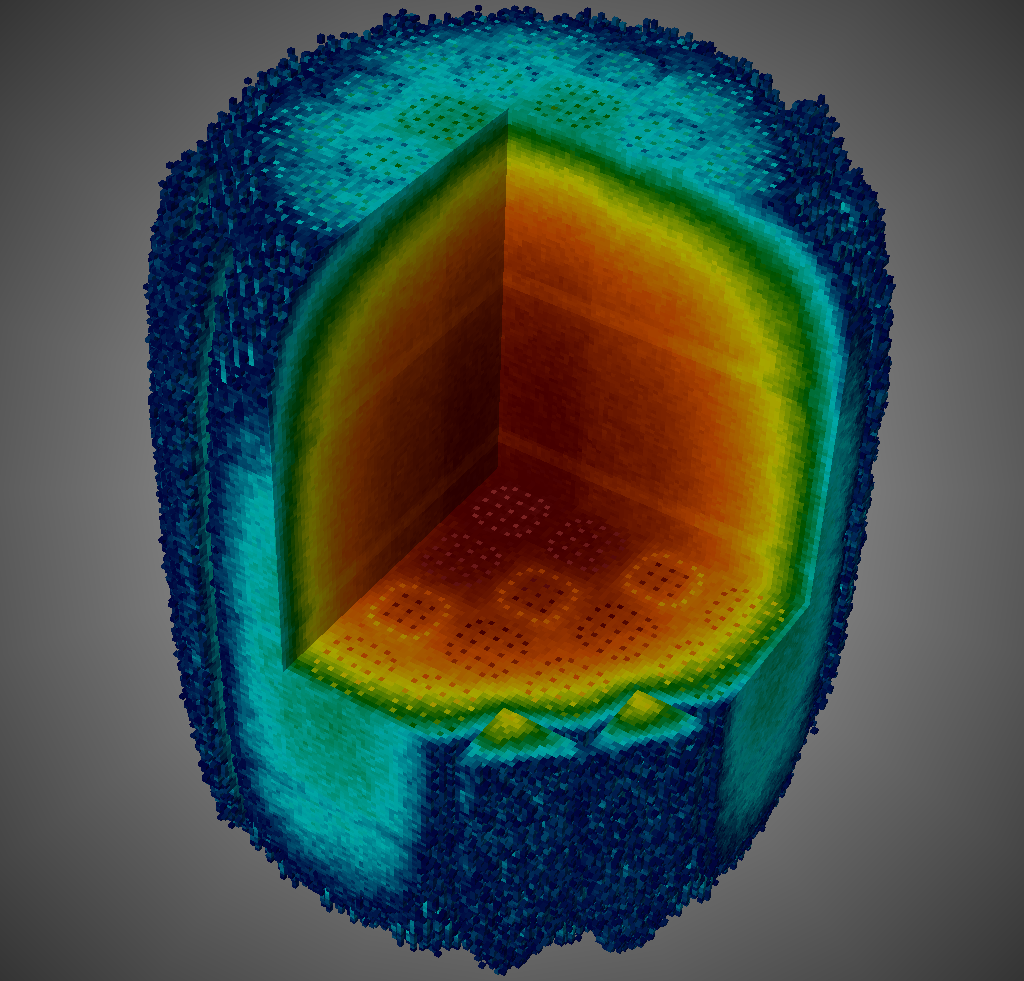
\includegraphics[width=2cm]{images/exasmr.png}
        \end{subfigure}
        \begin{subfigure}
           \centering
           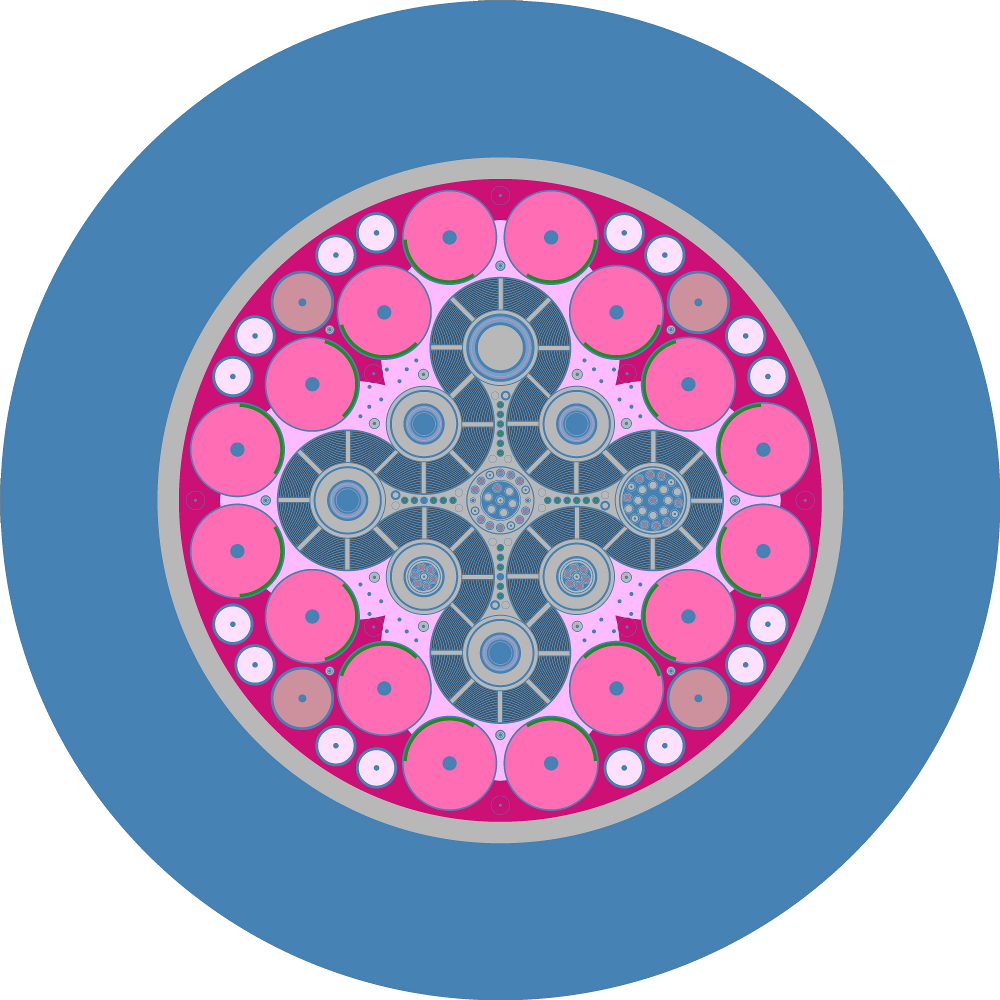
\includegraphics[width=2cm]{images/atr.png} 
        \end{subfigure}
        \begin{subfigure}
           \centering
           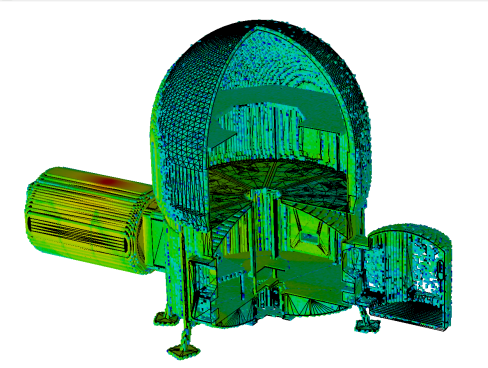
\includegraphics[width=2cm]{images/hab1.png} 
        \end{subfigure}
        \begin{subfigure}
            \centering
            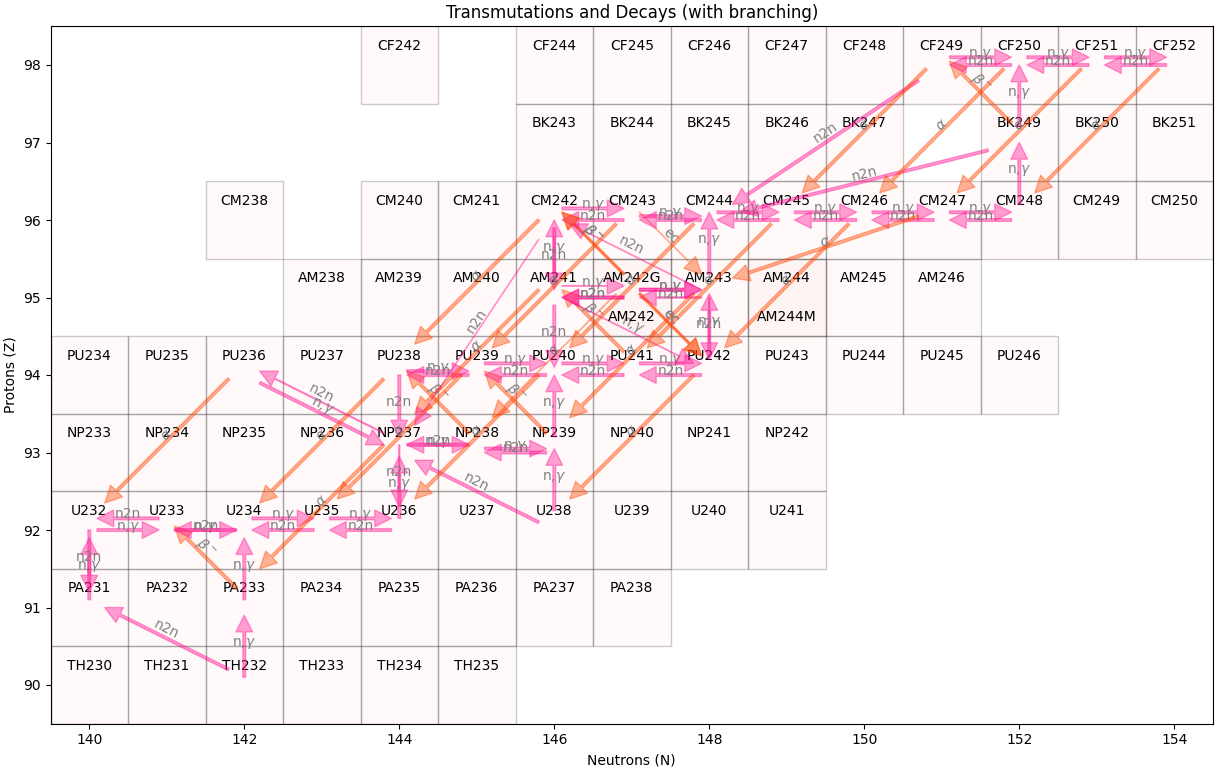
\includegraphics[width=4cm]{images/transmutation.png}
        \end{subfigure}
        {\tiny Sources: \cite{exasmr_fig},\cite{openmc_atr_slice},\cite{dagmc_nasa_module},\cite{armi_transmutation_fig}}
    \end{figure}
    \pause\medskip
    \begin{columns}
        \column[t]{5cm}
        \begin{itemize}
            \item Neutron transport
            \item Decay chains
            \item PRA
            \item Accident analysis
            \item {\bf Licensing activities}
        \end{itemize}

        \column[t]{5cm}
        Regulatory bodies will require new software features in order to effectively and efficiently perform licensing activities for the next generation of reactor deigns\cite{usnrc_nonlwr_2020-1}
    \end{columns}

    % add modeling + simulation looking figs here
\end{frame}

\begin{frame}
    \frametitle{Closed vs. Open source}
    \begin{columns}
        \column[t]{5cm}
        Closed codes
        \begin{itemize}
            \item Raises barrier to reproducing results in scientific literature
            \item Most closed codes have decades of development experience $\rightarrow$ more feature-rich, more code to maintain
            \item Educational/training resources may be more difficult to obtain
            \item May have to go through export control lisencing
        \end{itemize}


        \column[t]{5cm}
        Open codes
        \begin{itemize}
            \item Lowers barrier to reproducing results in scientific literature
            \item Most open codes have less than a decade of development $\rightarrow$ less feature-rich, more flexible when implementing new features
            \item Educational/training resources are easily accessible (if they exist)
            \item No need to go through export control
        \end{itemize}
    \end{columns}

\end{frame}

\begin{frame}
    \frametitle{Open source is the future for advanced reactor modeling}
    \Gls{IAEA} facilitated \Gls{ONCORE} initiative\cite{fiorina_initiative_2021}:
    \newline
    \newline
    \noindent ``ONCORE\ldots is an IAEA-facilitated international collaboration framework for the development and applictaion of open-source multi-physics simulation tools to support research, education, and training for analysis of advanced nuclear power reactors''\cite{iaea_open-source}

\end{frame}

\begin{frame}[t]
    \frametitle{How do you develop features in open codes?}

    There's no ``right'' way to do this, but there are useful conventions and concepts:
    \begin{itemize}
        \item Code standards (helps with formatting and automatic documentation)
        \item User and developer guides
        \item {\bf Version control}
        \item {\bf Open development}
        \item {\bf Automation}
    \end{itemize}
\end{frame}
